\chapter{SSaaS Applications}
\label{chap:apps}

As mentioned in previous chapters, many applications can utilize the
SSaaS model to allow users to reduce the trust they must place in any
single third party while still supporting popular use cases. This
chapter presents a discussion of common SSaaS application patterns as
well as a description of several specific SSaaS applications.

\section{Common Patterns and Challenges}

There are a number of common patterns and challenges that occur when
building SSaaS applications. This section discusses some of the more
prominent issues faced by SSaaS applications and proposed solutions to
each.

\subsection{SSaaS Metadata Storage}

Many SSaaS applications need to store metadata related to their
SSaaS-based operations. For example, ``key storage as a service''
(KSaaS) applications (e.g. client-side encryption, etc) require a
mechanism for mapping encrypted data to the key required to decrypt
it. Indeed, most SSaaS applications need a way to store useful
identifiers for each secret in order to facilitate the identification
of secrets by end users (e.g. a password manager needs to map services
to the corresponding secret/password). SSaaS applications must also
store the identity of the SSP (or SSPs) the user has selected for the
storage of their secrets in order to retrieve those secrets later.

Applications must decide how to best to store SSaaS-related metadata
in a manner that allows it to be quickly retrieved for the purpose of
identifying or accessing specific secrets. The need to maintain such
metadata is further complicated by the desire to support secret
sharing and syncing use cases. Both sharing and syncing operations
require the ability to share or sync the associated secret metadata in
addition to the secret itself. This requirement restricts the options
for storing metadata to designs that support sharing and syncing.

KSaaS-based encryption applications serve as a good example of the
kind of metadata SSaaS applications must maintain. Such split data/key
applications require the ability to map encrypted data to encryption
keys in a manner that allows the required key to be identified during
the decryption process.\footnote{This description uses encryption as
  an example of a split data/key SSaaS use case, but these ideas are
  applicable to data authentication use cases and other SSaaS-backed
  cryptographic primitives as well.}This mapping represents an
additional layer of persistent state that an application must
maintain. The loss of such a mapping would render any data stored by
the application useless since the application would no longer be able
to decrypt the data. It is worth noting that such key-mapping lookups
are predominately unidirectional: applications needing to lookup the
key corresponding to a known piece of data are far more common than
applications needing to lookup the data encrypted with a known
key. This is due to the fact that most applications (and their users),
natively operate in terms of data objects (e.g. files, photos, etc),
hiding the encryption from the user to increase usability. It is far
more natural for a user to request access to a piece of data for which
the application must lookup the corresponding key than it is for a
user to specify a key and need the applications to lookup the
corresponding piece of data.\footnote{The main exception to this rule
  is potential SSaaS management applications where a user may in fact
  wish to lookup a specific key and wish to ascertain which data it is
  used to protect.}

There are essentially three options for storing SSaaS metadata such as
that required to map keys to data (or vice versa). Each has pros and
cons. It is possible that applications may wish to combine several
techniques for the purpose of leveraging the strengths of each while
avoiding the flaws of any.

\begin{packed_desc}
\item[Out-of-Band Metadata:] An application may maintain an
  out-of-band mechanism for storing metadata. For example, an
  application could maintain a local database of data:key pairs. The
  advantages of such a solution are in its simplicity and ability to
  access metadata without needing to perform any form of remote API
  call to retrieve the corresponding secret or data. The ability to
  perform such local lookups may have performance benefits for certain
  applications. The biggest downside to this approach is that it
  requires the use of additional out-of-band mechanisms to share
  metadata with other users or sync it with other application
  instances. The need to implement such mechanisms increases the
  complexity of SSaaS applications. This approach also has the
  downside of increasing the risk of metadata loss. Storing the
  metadata via a separate mechanism unrelated to either the data or
  secret storage mechanism to which the metadata relates introduces an
  additional point of failure. As mentioned, the loss of metadata such
  as data-to-key mappings risks render both the corresponding data and
  keys meaningless.
\item[Key-Tied Metadata:] An alternative to maintaining out-of-band
  metadata storage is to store all required metadata via the SSP
  secret storage system. Such storage can be accomplished by allowing
  the application to provided arbitrary metadata fields associated
  with each secret or by allowing the application to encode metadata
  into the secret ID itself. For example, an application could store
  the identity of the data to which a given key corresponds as a
  metadata attribute of the key itself. This has the benefit of
  avoiding the need for an out-of-band database, and has a graceful
  failure mode in which metadata is only lost if the secret to which
  it corresponds is also lost -- in which case the metadata would
  likely be useless anyway. The main downside to this approach is that
  it is not well optimized for computing data-to-metadata lookups such
  as those required to discover the ID of the decryption key for a
  piece of encrypted data. Such lookups require an inefficient
  exhaustive search of all secrets until the one with the required
  metadata value is found.
\item[Data-Tied Metadata:] An application can also invert the idea of
  a key-tied metadata by storing all SSaaS metadata with the data
  itself. This might be accomplished either by leveraging data-linked
  metadata fields (e.g. the extended attributes offered by many file
  systems) or by writing additional data to the storage medium itself
  (e.g. using a ``header'' structure that precedes each chunk of
  encrypted data and identifies the key required to decrypt the
  data). Like key-tied metadata, data-tied metadata avoids creating an
  additional point of failure by linking metadata storage to the data
  that depends on it. Furthermore, data-tied metadata can perform
  constant-time data-to-metadata lookups. This makes such techniques
  well optimized for encryption systems requiring quick data-to-key
  lookups. Furthermore, such metadata storage adapts well to sharing
  and syncing use cases since any mechanisms already in place to share
  or sync the underlying data (e.g. Dropbox) will also share and sync
  the associated SSaaS metadata. The main downside to data-tied
  metadata storage is the need to perform an exhaustive search to
  compute key-to-metadata lookups. But since such lookups tend to be
  rare, this deficiency may not be widely noticed.
\end{packed_desc}

In many SSaaS applications, it is likely desirable to use a
combination of these techniques. For example, an application could use
both key-tied and data-tied metadata storage to ensure both constant
time data-to-key as well as constant time and key-to-data
lookups. Furthermore, an application could also use a local metadata
database as a high speed cache for common metadata lookups, avoiding
the need to query the data storage medium or SSP to access metadata in
many instances. The downside to a combined approach is the additional
complexity required keep the multiple metadata stores internally
consistent. Such challenges, however, are common in data storage
applications and have a variety of general purpose solutions.

\subsection{Data Granularity}

In addition to metadata storage for maintaining data-to-key mappings,
encryption and authentication based SSaaS applications must also
tackle the decision of at which granularity they wish to encrypt or
authenticate data. Traditionally this decision is driven by
complexity, performance, and access control
requirements~\cite{li2013}.  SSaaS-backed applications are no
exception.

As an example, consider a disk encryption system. This system could
encrypt data in a variety of ways: it could encrypt individual disk
blocks, it could encrypt individual files, or it could encrypt
individual directories and all the files they contain. Encrypting
individual disk blocks using a single key tends to be fast and simple,
but makes controlling access to specific files, as opposed to the
entire disk, difficult. The higher-level file and directory encryption
provides finer grain control over access (e.g. by using separate
encryption keys for each file), but incurs additional file system
overhead. In general, lower level mappings are going to be faster, but
lack support for finer grained access control. Higher level systems
are slower, but have more flexible access control options.

The SSaaS model complicates this further by adding additional overhead
to the key retrieval phase of any encryption or data authentication
operation. Thus, a block-level disk encryption system that uses a
single key to protect an entire disk incurs minimal SSaaS overhead
since it requires only a single SSP key lookup when the disk is first
accessed. But such a setup would limit the user to a single set of
SSP-enforced access control rules for the entire disk. Per-file
encryption, on the other hand, incurs significantly more (but still
manageable) overhead by required an SSP key lookup for each file open
operation. File mappings, however, allow the user to set individual
access control rules for each file.

There exist additional encryption granularity options. For example,
the SSaaS model could be used to store a separate key for each
individual hard disk sector. Such a setup would allow potentially
interesting methods of per-sector disk access control, but would also
significantly increase disk latency by requiring a round trip SSP key
lookup for each individual sector. Such a design could incur thousands
of lookups to access a single file. Developers must consider the
additional SSP-overhead the SSaaS model entails when deciding on the
level of granularity required for a given encryption application.

\section{Use of SSaaS Libraries and Utility Programs}

One of the benefits of the SSaaS model is the use of a standardized
protocol providing access to secret storage functionality. As
mentioned in Chapter~\ref{chap:ssaas}, this standardization has
numerous benefits, most notably the encouragement of SSP
competition. An additional benefit of standardization is the ability
to use standard SSaaS libraries and utilities across a range of SSaaS
applications. Such systems reduce the complexity of each individual
SSaaS application by allowing common SSaaS tasks to be abstracted into
dedicated libraries or utilities.

The implementation of SSaaS client functionally will often be non
trivial, especially when considering the need for such applications to
support the ability to shard secrets across multiple SSPs. The
potential complexity of such solutions likely calls for the creation
of a standardized SSaaS client libraries that can be utilized by
multiple applications. Such a library avoids the need for each SSaaS
application to reimplement SSaaS API communication primitives
directly. Similar to the manner in which most applications use common
cryptography libraries to avoid needing to reimplement cryptographic
code, SSaaS applications can use common SSaaS libraries to simplify
their integration with the SSaaS ecosystem.

Furthermore, it may also be desirable to create common SSaaS
management utilities. Many of the SSaaS-related management features --
e.g. setting up access control requirements, checking audit logs, etc
-- are common across all SSaaS applications. It is thus desirable to
offload such functionality to a general SSaaS management utility in
cases where such functions need not be tightly coupled with a given
SSaaS-backed application. This offloading would allow SSaaS-backed
applications to focus purely on the secret storage and retrieval side
of the SSaaS API while dedicated management utilities handle the
access control and auditing side of the SSaaS API.

\section{Storage}

One of the primary applications of the SSaaS model is to secure
storage systems, both local and hosted. These applications are all
variations on the previously discussed encrypted data with
SSaaS-backed keys model
(Chapters~\ref{chap:intro},~\ref{chap:challenges},
and~\ref{chap:ssaas}). In such applications, local programs handle the
encryption and verification of data, storing only encrypted data with
third parities and/or on high risk devices while storing the
associated encryption keys with one or more SSPs.

\subsection{Cloud File Sync/Storage}

\begin{figure}[t]
  \centering
  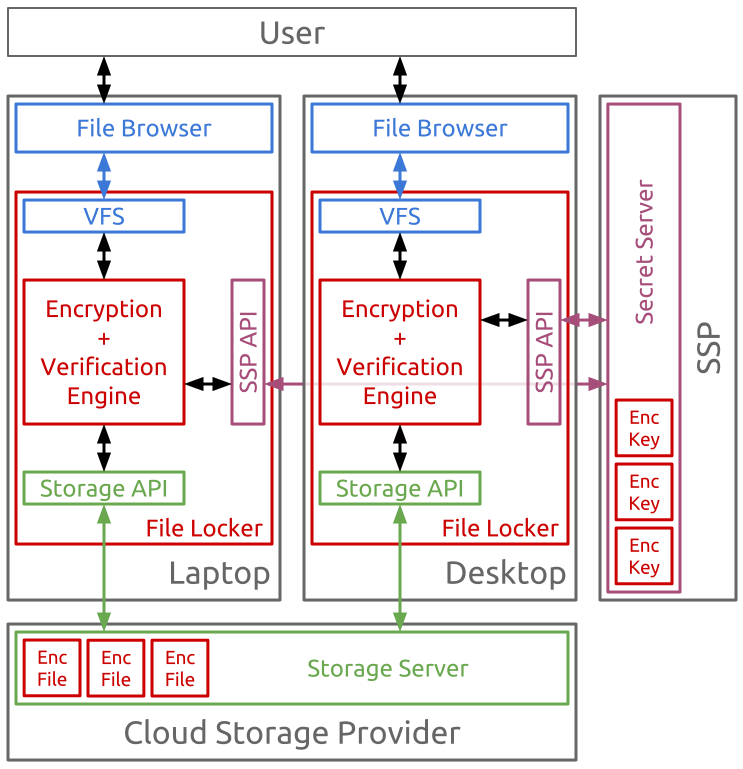
\includegraphics[height=200px]{./figs/out/App-FileLocker.pdf}
  \caption{SSaaS-Backed Cloud File Locker System}
  \label{fig:apps-filestore}
\end{figure}

Building on the original motivating example in this dissertation,
i.e. using Dropbox without trusting Dropbox,
figure~\ref{fig:apps-filestore} illustrates an SSaaS-backed secure
cloud storage application. As in the general storage case, this
application involves applying client-side encryption/decryption
(e.g. using AES~\cite{nist2001}) and signing/verification (e.g. using
CMAC~\cite{dworkin2005}) on every read and write to a third party
backed data store. The third party data store holds only encrypted and
authenticated data, ensuring that the third party need not be granted
the Access (\emph{R}-type) and Manipulation (\emph{W}-type)
capabilities.

In order to ensure that users can still share data with other users
and sync it across devices, the application stores all required
encryption and authentication keys with one or more SSPs. When a user
wishes to sync data to a new device, they grant said device access to
the necessary keys via their SSP's management interface. The new
device can then download the encrypted files from the minimally
trusted storage provider and decrypt/verify them using the keys
provided by the SSP. Device authentication can be provided via
certificates, shared-secrets (e.g. passwords), or contextual
information. When a user wishes to share data with another user, they
grant the new user access to the encrypted data via the storage
provider's normal sharing mechanisms. They then also grant the new
user access to the necessary keys via the SSP's management
mechanisms. The user can now download the data from the storage
provider and decrypt and verify it with the keys from the SSP. As in
the multi-device sync case, authentication may be performed via a
variety of mechanisms, allowing the data owner to select the
authentication primitives best suited for a given situation.

This type of application overcomes the traditional deficiencies of
secure cloud-based data storage. It minimizes trust in the third party
storage provider by only granting them access to encrypted and
authenticated data. It also maintains support for the multi-device and
multi-user use cases traditionally associated with cloud-backed data
storage through the use of SSPs for key storage. The SSaaS model
allows users to enhance their privacy and security by reducing
exposure to third parties without incurring additional usability
burdens or denying access to desirable features.

\subsection{Server Data Encryption}

Beyond consumer-oriented encryption systems, there is a strong case
for using SSaaS-backed encryption systems for datacenter-based
servers. Leveraging virtual (as well as physical) servers hosted in
cloud data centers is an extremely popular deployment
method. Unfortunately, as mentioned in Chapter~\ref{chap:challenges},
an administrator's lack of physical access to such servers makes it
difficult to utilize privacy-enhancing technologies like Full Disk
Encryption (FDE) or file-system level encryption. In the FDE case,
users are generally required to provide some form of decryption
passphrase or physical dongle at boot-time in order to securely
bootstrap the system. Similarly, even in the file-system level
encryption case, encryption systems generally require some form of
interactive mechanism to provide the necessary security passphrase to
decrypt the system. Since administrators generally lack both physical
access to datacenter-based servers as well as an interactive presence
on such servers, using traditional encryption systems with most cloud
servers remains difficult, if not impossible.

These deficiencies can largely be resolved via SSaaS-backed encryption
systems -- either full disk or file-system oriented. Using SSaaS, a
user can configure each server to store their file encryption and
verification keys with an SSP (or SSPs). Each server can then request
the keys from the SSP at boot or on access to an encrypted file. Such
an application can leverage non-interactive authentication techniques
such as the contextual techniques discussed in~\cite{hulsebosch2005}
to achieve autonomous operation (e.g. does the system expect a server
to be rebooted at a certain time of day?). In more sensitive
situations, the SSP's access control system could even keep the user
in the loop by asking the user to provide a passphrase or decryption
approval via text message or similar out-of-band real time
communication method each time key access is required.

Such systems would allow users to store sensitive data on servers
while minimizing the degree of trust they must place in third party
data center hosts. In this model, cloud servers would store all data
in an encrypted form, ensuring that a physical search of the
underlying storage medium or other interference from the data center
host would not be easy. Encrypted data would be decrypted on-demand,
making it very difficult for the data center host to access it without
employing high degrees of subterfuge. Even in cases where the data
center host does manage to leverage their control of the underlying
physical systems to trick an SSP into providing decryption keys, the
SSP would still be able to log and audit the event -- making it
extremely difficult for a data center host to access secure user data
in an undetectable manner.

SSaaS-backed, server-based encryption efforts provide a mechanism to
significantly decrease the amount of trust developers (and by proxy,
their users) must place in the providers of hosted server
infrastructure without significantly raising the cost or overhead of
leveraging such infrastructure.

\subsection{Mobile Device Encryption}

The SSaaS model also provides benefits for the protection of local
storage. Mobile devices such as phones, tablets, and laptops store
huge quantities of personal information. Yet these devices are more
prone to theft and loss than traditional computing systems such as
desktops and servers. The encryption and protection of such devices is
thus a high priority when working to increase the privacy and security
of users.

Traditional device encryption systems have become prevalent in Android
and iOS-base mobile devices~\cite{ars-android-encrypt,
  ars-ios-encrypt}. Such systems are useful for ensuring that
device-stored data can not be accessed when devices are shutdown or
(when properly designed) locked, but they do little to protect data
when the phone is (or has recently been) in use. Furthermore, the
encryption keys for such systems are stored locally (often via an HSM)
and are generally only protected with a short pin or passphrase.

Mobile encryption systems could be converted to an SSaaS model where
the keys are stored with one or more SSPs, providing a number of
benefits over local key storage. First, since keys are stored
off-device in an SSaaS-backed encryption system, it is easy to revoke
access to the keys remotely in the event that a device is lost or
stolen, ensuring that an attacker can not guess a user's PIN and
access their data. Second, such a system could be used to protect
individual pieces of data separately, as opposed to the current
practice of unlocking all data when the device starts up. In doing so,
it would be possible for a user to set per-app access control rules
with their SSP, effectively reducing the trust the user must place in
the third party apps they install on their devices. Users could
leverage the SSaaS model to audit all app data access and limit apps
to accessing only the data they are expected to need. Finally, an
SSaaS system would provide more flexible access control semantics on
mobile devices than the standard Everything/Nothing access model
common today. For example, an SSaaS system could be set up to provide
keys to one set of data to User A while providing keys to a separate
set of data for User B -- effectively protecting per-user data on
multi-user devices. Similarly, an SSaaS system could be configured to
provide access overrides in specific situations -- e.g. allowing an
authorized secondary user to access the device and the data it stores
in the event that the primary user becomes incapacitated (e.g. similar
to the functionality provided by Google's Inactive Account
Manager~\cite{atlantic-google-iam}, but with cryptographic
guarantees).

\subsection{Personal Data Repository}

\begin{figure}[t]
  \centering
  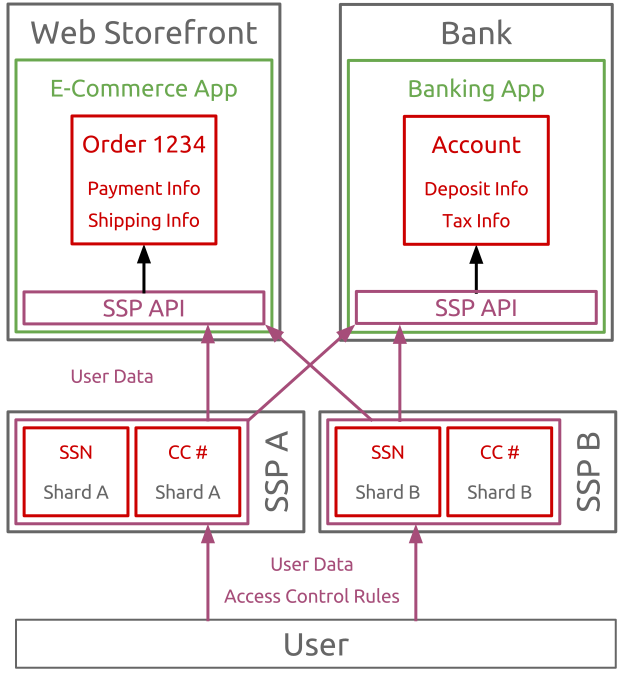
\includegraphics[height=200px]{./figs/out/App-DataRepo.pdf}
  \caption{SSaaS-Backed Personal Data Repo}
  \label{fig:apps-datarepo}
\end{figure}

Moving past encrypted storage applications, users could also leverage
the SSaaS model to create a dedicated repository of personal info (e.g
SSN, address, etc). Requiring users to enter personal data on various
websites is a common user requirement for placing orders, creating
accounts, etc. This practice is undesirable for several
reasons. First, it is highly burdensome: users are continually forced
to reenter the same info again and again and must ensure they keep it
up to date across multiple sites. Second, it distributes a lot of
sensitive user data across a large number of actors in a manner that
is very difficult for a user to track or control. Instead, an
SSaaS-backed data repository would allow a user shard their data
across several SSPs and then point websites that require it directly
at the SSPs themselves. The user would then specify Access Control
rules with each SSP allowing specific websites access to the minimum
data they require.

Not only does this approach provide a central repository where the
user can enter personal data and keep it up to date (e.g. when moving
or changing their name), but it also allows the user to limit each
site's access to only certain data and provides an audit trail for the
user to track exactly which sites have accessed which
data. Figure~\ref{fig:apps-datarepo} illustrates such a use case. In
this case, as opposed to the previous applications, the user is
storing sensitive user data directly with their SSPs. As such, it will
be important to shard the data across multiple SSPs in order to
minimize the trust they must place in each individual SSP.

Such applications would go a long ways toward minimizing the amount of
sensitive personal data users have stored with large number of third
parties in favor of concentrating it on only a handful of SSPs. Doing
so both reduces the trust users must place in any single SSP and
ensures the data is being stored with parties better incentivized to
protect it (see the discussion in Section~\ref{chap:ssaas:trust}).

\section{Communication}

\begin{figure}[t]
  \centering
  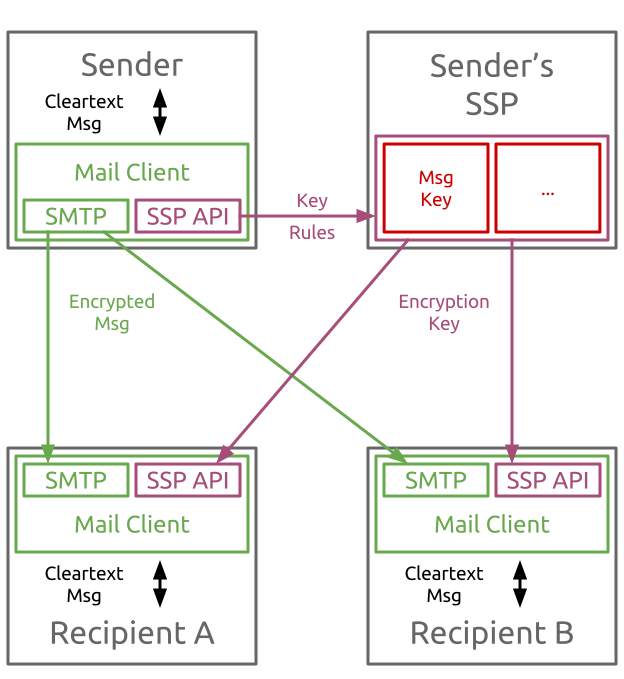
\includegraphics[height=200px]{./figs/out/App-SecureEmail.pdf}
  \caption{SSaaS-Backed Secure Email System}
  \label{fig:apps-secureemail}
\end{figure}

The applications of SSaaS are not limited to data storage. Another
potential area of application involves secure communication between
two or more parties. Such secure messaging systems are in growing
demand, especially after the Snowden revelations related to U.S.
Government monitoring of email and associated digital communication
systems~\cite{gellman-muscular, greenwald-collect,
  greenwald-prism}. While solutions like GnuPG~\cite{gnupg} allow
users to secure the contents of their mail, their complexity tends to
limit their use to a small subset of advanced
users~\cite{green-challenge, whitten1999}. The use of SSPs and the
SSaaS model could simplify the secure communication paradigm.

Figure~\ref{fig:apps-secureemail} illustrates a potential SSaaS secure
communication use case. In this application, a user's mail client
would encrypt the contents and subject of a user's email with a
locally-generated single-use symmetric encryption key. The client
would than upload this key to the user's SSP where the user would
specify that their intended recipients should have read access to the
key. The user could then send the encrypted mail. When received, the
recipient's mail client would request the required key from the
sender's SSP, providing appropriate credentials to prove their
identity in the process. This system would be capable of supporting
multi-recipient systems like newsgroups and would also allow the user
to grant read access to additional users after the fact (e.g. should
the recipient wish to forward the email to an additional trusted
party), both capabilities that traditional public-key based email
encryption systems struggle to support. Similar applications could be
designed for real-time communication such as chat.

As in previous cases, third party trust can be minimized by sharding
keys across multiple SSPs. Furthermore, such systems could guarantee
some degree of forward secrecy by having the SSP automatically expire
and delete keys after a certain period of time -- something that
traditional email encryption systems fail to support. Such designs
have the potential to raise the default level of security inherent in
mass digital communication without significantly inconveniencing users
or requiring the replacement of existing protocols.

\section{Authentication}

SSaaS also has applications in the authentication realm. Cryptographic
authentication systems (i.e. certificate-based authentication) are
considered to be some of the most secure forms of digital
authentication -- far better than more commonly deployed shared-secret
(i.e. password) authentication systems. Whereas shared secret
authentication relies on both the user and the verifier (e.g. server)
knowing a common secret such as a passphrase, certificate-based
authentication systems rely on a user to be able to cryptographically
prove they possesses the private key corresponding to a specific
public key. Such systems have a range of applications, from websites
to servers and workstations. For example, SSH~\cite{ylonen1996}, one
of the more common remote-access protocols for Unix-like computing
systems, uses key-based authentication on both the server (where keys
provide server verification) as well as on the client (where keys
authenticate users instead of passwords). SSH is thus a useful example
to demonstrate the potential benefits of the SSaaS model to
authentication systems. SSaaS can provide usability and security
benefits to SSH on both the client and server.

\subsection{SSH Agent Key Management}

\begin{figure}[t]
  \centering
  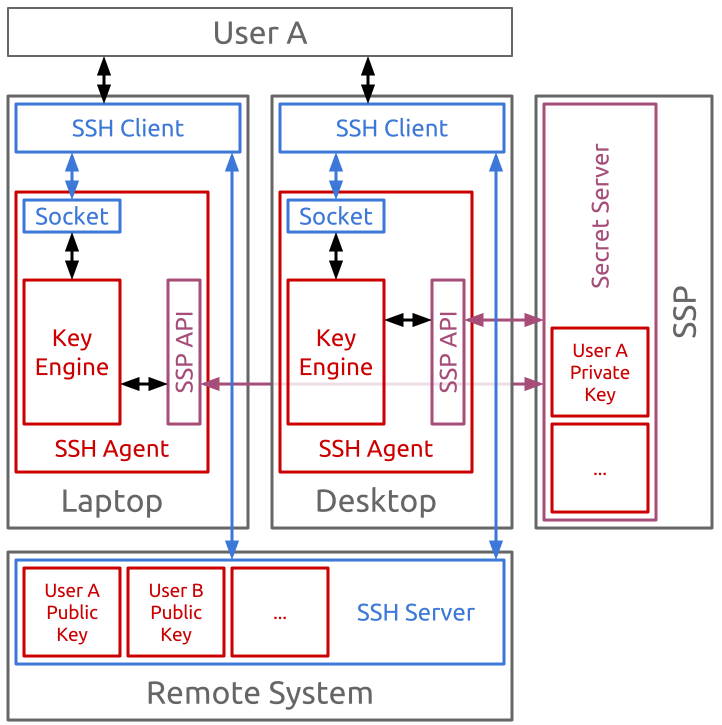
\includegraphics[height=200px]{./figs/out/App-SSHAgent.pdf}
  \caption{SSaaS-Backed SSH Agent}
  \label{fig:app-sshagent}
\end{figure}

The management of private cryptographic keys has long been a challenge
for users. To help mitigate this challenge, the systems community has
developed the concept of an ``agent'' program. Agent programs sit
between the user and an authentication system, providing the required
cryptographic keys on the user's behalf to the authentication system
when required~\cite{cox2002}. Agents are commonly used with popular
computing utilities like SSH~\cite{ylonen1996} and
GnuPG~\cite{gnupg}. Unfortunately, existing agent solutions are
designed for legacy usage models: single-device, non-portable desktop
environments. They do not provide a mechanism for managing private
keys across multiple devices, securing keys if the associated device
is lost or stolen, or managing keys for a large group of users across
an organization.

An SSaaS-backed agent can overcome the locality and management
challenges associated with traditional cryptographic agent
programs. Figure~\ref{fig:app-sshagent} shows the basic design for an
SSaaS-backed SSH-agent. Instead of storing private keys locally, the
agent would defer private key storage to one or more dedicated
SSPs. When the agent requires the user's private keys, it requests
them from the SSP. Thus, the user and any associated agent programs
are able to securely access the necessary private keys from multiple
devices (e.g. laptop, desktop, tablet). Furthermore, if the user ever
loses one of their devices, they can greatly reduce the risk of
exposing any of their private keys by revoking the lost device's
access to the off-site SSaaS data (e.g. similar to~\cite{geambasu2011}
and~\cite{tang2012}). Such a system also allows large organizations to
manage SSH or other cryptographic keys for all their users from a
centralized SSaaS management application.

Divorcing private SSH key storage from local devices opens up a range
of use case possibilities, increases security by keeping keys off of
frequently lost or stolen portable devices, and relieves the user of
the usability overhead required to manually manage their private keys.

\subsection{SSH Server Key Management}

\begin{figure}[t]
  \centering
  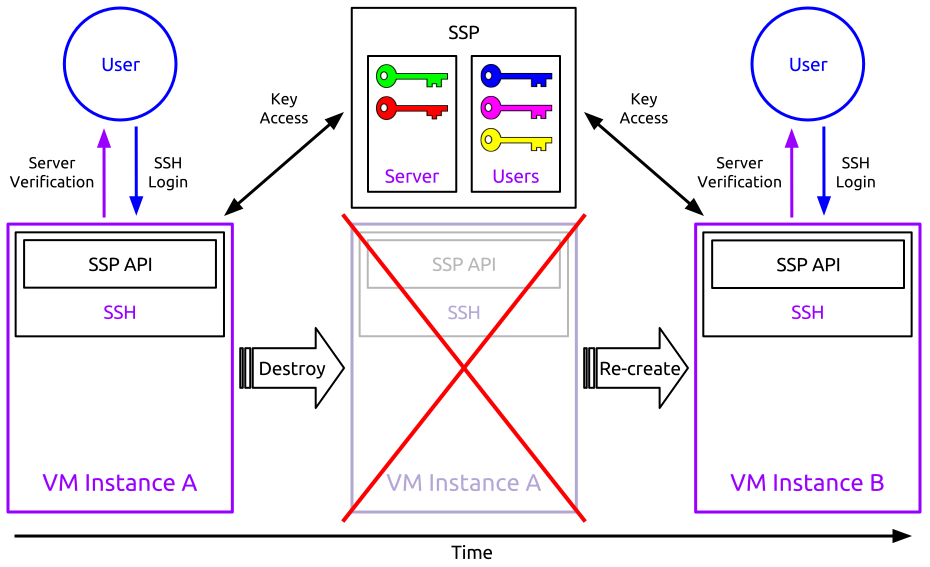
\includegraphics[height=200px]{./figs/out/App-SSHServer.pdf}
  \caption{SSaaS-Backed SSH Server Key Management}
  \label{fig:apps-sshserver}
\end{figure}

Similarly, the SSaaS model can provide benefits when applied to the
server side of SSH. An SSH server must manage both a server key pair,
used to prove the server's identity to a user and to bootstrap the
negotiation of a session key, as well as a list of user public keys
for any users granted server access. Unfortunately, managing both sets
of keys manually poses a number of challenges. Integrating server-side
SSH key management with an SSaaS system can help alleviate these
challenges.

In the server key case, the ephemeral nature of modern IaaS-based
systems causes issues with locally manged keys. For instance, what the
user perceives of as a single server may actually be multiple
load-balanced servers, or may be a single virtual server that is
destroyed and recreated frequently in response to upgrades and changes
in demand. In either case, it is important that the user be able to
properly authenticate that the server they are accessing is in fact
the correct server and not a malicious man-in-the-middle
attacker. Unlike SSL/TlS, however, SSH does not rely on a central
certificate authority structure for the verification of keys. Instead
it uses a ``trust on first use'' (ToFU) model that fingerprints a
server key the first time the user connects and then assumes that this
key will remain associated with a given server address
indefinitely. If an ephemeral cloud server generates a new server SSH
key each time it is recreated, or if multiple logically equivalent,
load-balanced servers all have different SSH keys, a user will be
unable to verify that the server is equivalent to the one they
originally accessed. This issue could be overcome by storing the SSH
verification keys for a server with one or more SSPs as shown in
Figure~\ref{fig:apps-sshserver}. Then, when a server is recreated, or
when a single logical server is balanced between multiple instances,
it still has access to the same SSH keys originally in use, ensuring
that previous users can properly authenticate the server as valid.

The server's list of authorized user keys poses similar
challenges. These lists contain the public keys of all users
authorized to access a given server. Maintaining such lists across
large numbers of servers, and ensuring they stay up to date even as
individual server instances are added, removed, and upgraded is
challenging. Failing to properly manage such lists can either lead to
legitimate users being locked out of systems, or worse, allowing
illegitimate users (e.g. a previous employee) to access systems they
should not. Indeed, such misconfiguration errors are one of the
leading causes of security failures today~\cite{bishop1996,
  kerravala2002}. Centralizing the management of such authorized keys
lists with an SSP allows administrators to manage and audit server
access across a wide collection of infrastructure from a single
place. This solution is the SSaaS equivalent of cloud user management
solutions such as JumpCloud~\cite{jumpcloud}. But unlike existing
services, an SSaaS-backed SSH user management system avoids trusting
any single third party by leveraging the key-sharding possibilities
available in an SSaaS ecosystem.

Both of these setups illustrate the benefits an SSaaS system can
provide to common authentication and user management problems in cloud
servers. In many ways, SSaaS represents a more secure variant of
traditional configuration management solutions such as
Chef~\cite{chef}, Salt~\cite{salt}, or Puppet~\cite{puppet}. But
unlike such solutions, the SSaaS model is designed with the security
and privacy of the configuration data it stores as a first principle,
not a secondary concern.

\section{Dedicated Crypto-Processor}

\begin{figure}[t]
  \centering
  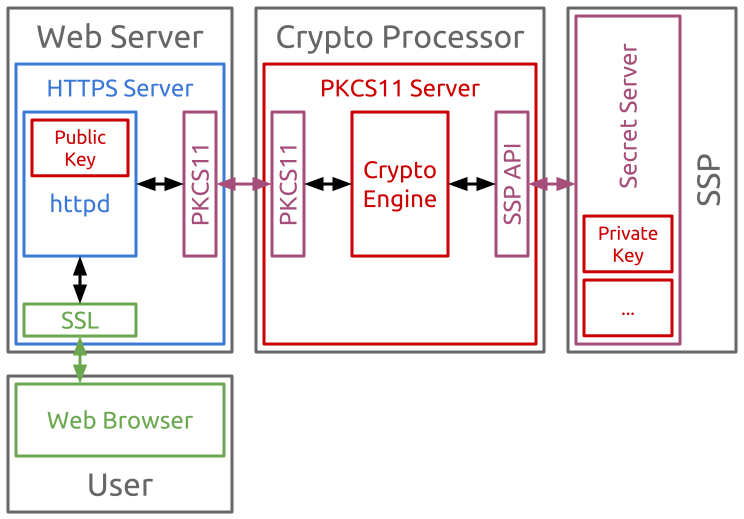
\includegraphics[height=200px]{./figs/out/App-PKCS11.pdf}
  \caption{SSaaS-Backed Dedicated Crypto-Processor}
  \label{fig:app-pkcs11}
\end{figure}

The recent Heartbleed bug~\cite{heartbleed} exposed one of the main
risks of embedding cryptographic secret storage within the
applications requiring access to these secrets: when applications
break, they also risk exposing access to the private keys stored in
the same memory segments. The Heartbleed fallout has forced developers
to reevaluate whether or not giving public-facing services direct
access to cryptographic keys is a good idea. There has long existed an
alternative: using a hardware security module (HSM) to perform
dedicated crypto-processing and key storage on behalf of other
services. Such systems ensure that cryptographic keys are never
exposed outside of the secure hardware module. Programs communicate
with the HSM via a standard protocol like
PKCS\#11~\cite{pcks11-standard}. In such systems, an application sends
the HSM clear-text data to encrypt and gets back the encrypted
ciphertext in return. Unfortunately, most existing HSM solutions don't
scale to the performance levels required by high-volume services. This
has led some to suggest moving to a software-based ``HSM''
model~\cite{lorier-pkcs11}. Such ``softHSM'' systems would ensure
cryptographic keys remain stored in separate isolated memory spaces
while also out-performing traditional HSM systems.

A software-based dedicated crypto-processing system is an ideal use
case for an SSaaS-backed system. Figure~\ref{fig:app-pkcs11} shows the
potential design of such a system. Here, a Secret Storage Provider
supplies the back-end key storage for a dedicated crypto-processing
server which performs cryptographic operations (e.g. SSL encryption
and authentication) on behalf of a web-server. In this setup, the
web-server never accesses any private cryptographic keys directly,
mitigating one of the major risks Heartbleed exposed. Furthermore, the
logically centralized nature of an SSaaS SSP allows dedicated
crypto-processing servers to scale horizontally (e.g. multiple
load-balancing instances) as demand requires: storing all keys via one
or more SSPs allows new crypto-processing instances to immediately
access these keys without the need to utilize ad-hoc key-syncing or
configuration management interfaces. Finally, the SSP's auditing
functionality ensures that one always knows which keys have been
accessed by which systems, placing hard bounds on what an attacker may
or may not have had access too: a luxury that Heartbleed-prone servers
did not have.

An SSaaS-backed crypto-processor design combines the benefits of a
dedicated crypto-processor with the third party trust limiting nature
of the SSaaS model. This combination allows for scalable high speed
cryptographic processing without placing a high degree of trust in any
single system or party.

%%  LocalWords:  SSaaS CMAC SSPs SSP's SSP FDE iOS Repo Snowden IaaS
%%  LocalWords:  JumpCloud Heartbleed PKCS softHSM KSaaS FP ToFU
%%  LocalWords:  passphrase
